\section{Analysis and Findings}

The dataset includes voice measurements from 31 individuals, 23 with
Parkinson's disease, across 195 recordings. The recordings are labeled as 0 for
healthy and 1 for Parkinson's. Features include: absJitter, apq, apq3, apq5,
avFF, dda, dbShimmer, ddp, D2, DFA, HNR, lShimmer, maxFF, minFF, NHR,
percJitter, PPE, ppq, rap, RPDE, spread1, and spread2.

First, we conducted an exploratory analysis of the dataset. No missing values,
NaN entries, or duplicates were found. We then performed the following
preprocessing steps:

\begin{itemize}
	\item \textbf{Renaming:} We designed the function \texttt{rename()} to
	      standardize column names. It takes a DataFrame and a dictionary of correct
	      names as inputs, making the dataset easier to use.

	\item \textbf{Outlier Removal:} We used then function \texttt{outliers()}
	      based on interquartile range (IQR) method \((Q3 - Q1)\) to identify
	      outliers. These were replaced with the mean of non-outlier values within
	      each subject. This avoids mixing healthy and Parkinson's data, assuming
	      values within a subject are consistent.

	\item \textbf{Aggregating:} We used \texttt{aggregate()} to group the
	      DataFrame by \texttt{subject\_id} and compute the mean for each group. This
	      method captures the average feature values across trials for each individual.

	\item \textbf{Normalizing:} Using the function \texttt{normalize()}, we
	      applied Min-Max scaling:

	      \begin{align} x_{\text{normalized}} = \frac{x - \min(x)}{\max(x) - \min(x)}
	      \end{align}
\end{itemize}

For the KNN model, we conducted dimensionality reduction, focusing on
parameters related to fundamental frequency, jitter, and shimmer. The
\texttt{collinearity()} function calculated correlations within each feature
group and identified the least correlated pairs. To retain a feature, we
compared its correlation with all other features. A scoring system assigned
higher scores to features with lower overall correlation. Features with higher
scores were kept, while others were removed.

\cref{fig:fig2} shows correlations for fundamental frequency features. As you
can see, since these metrics are relative to the same measure, it makes sense
that they show some sort of correlation between them.

\begin{figure}[H]
	\centering
	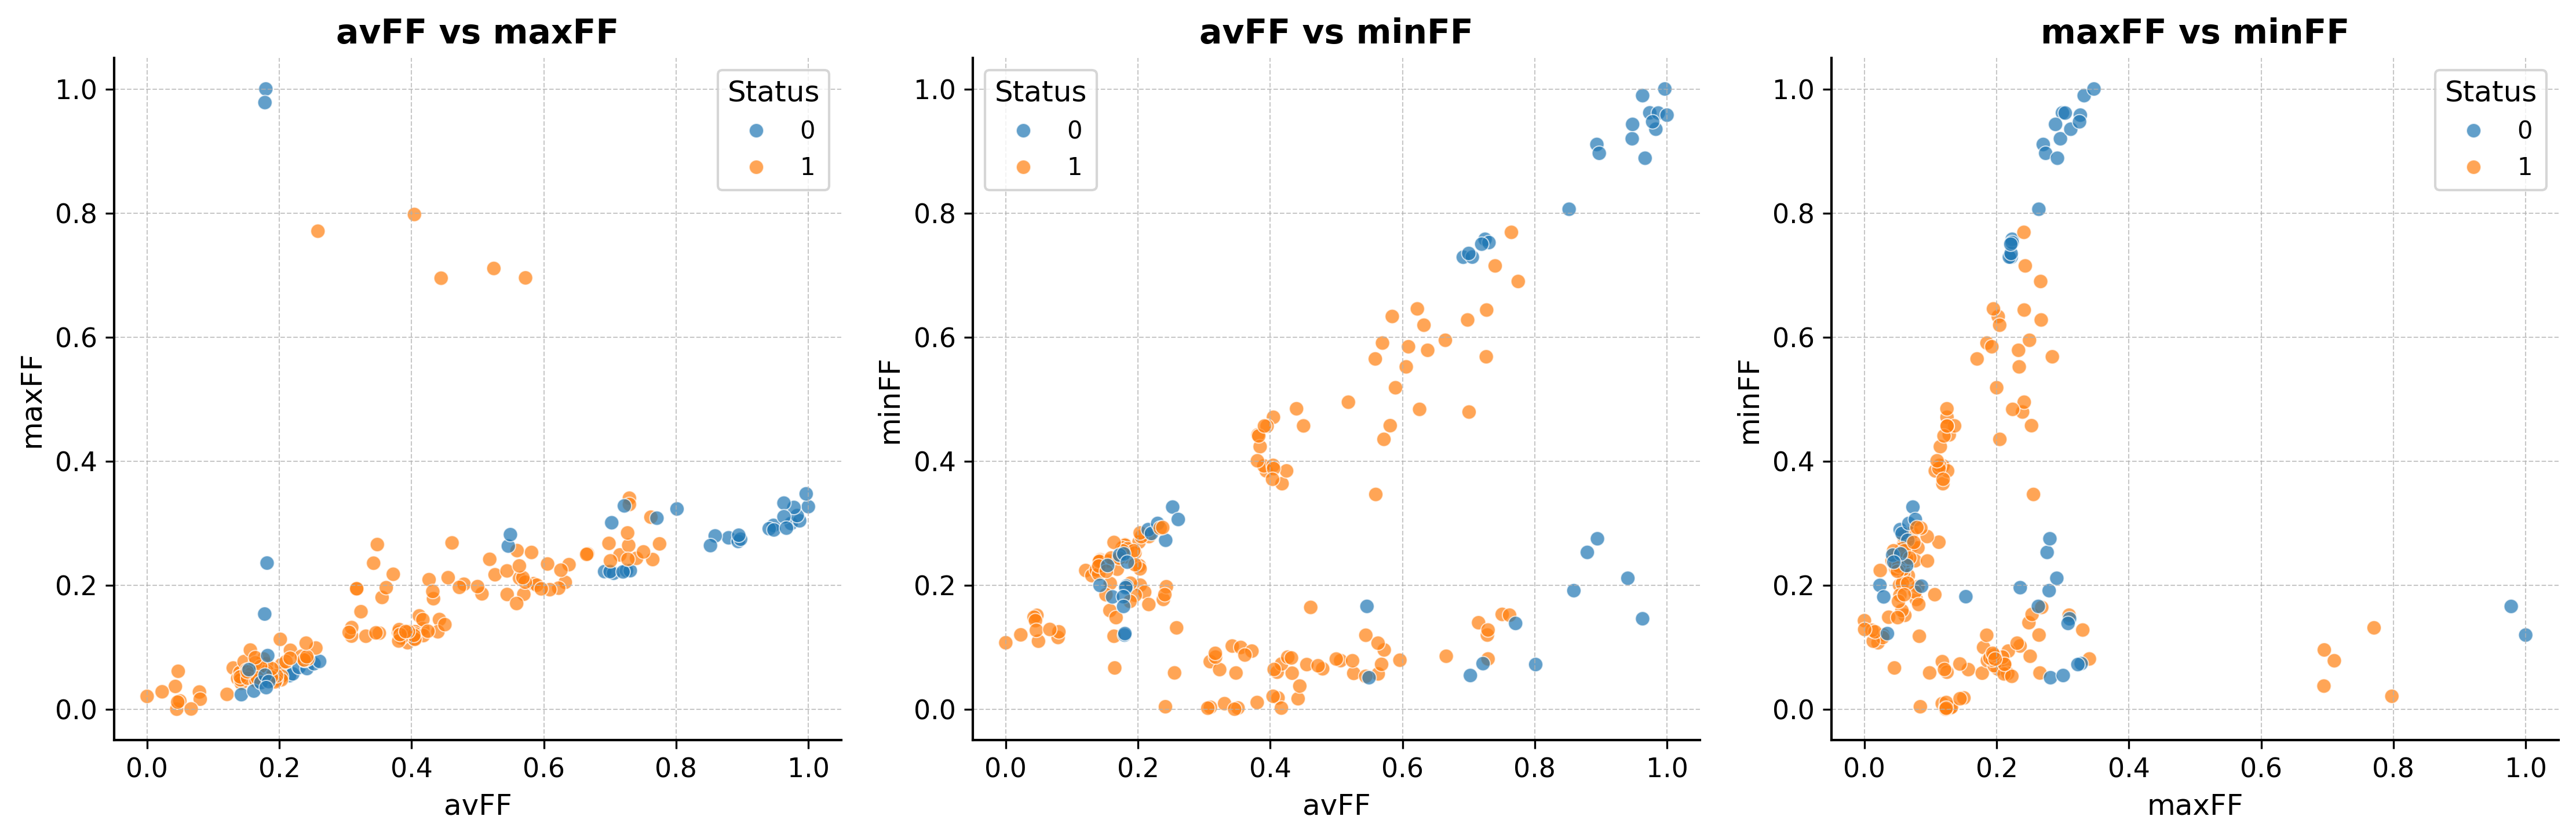
\includegraphics[width=0.99\textwidth,height=6cm]{../images/feature_selection/fundamental_frequency.png}
	\caption{Correlation among fundamental frequency-related parameters.}
	\label{fig:fig2}
\end{figure}

The final selected features to train the model were: absJitter, apq, D2, DFA,
HNR, maxFF, NHR, PPE, RPDE, spread1, spread2.

For validation, the data was split into 70\% training and 30\% testing. To
optimize the hyperparameter \(k\), we selected the value where testing and
training accuracy were similar. The intersection of these points was found
using linear interpolation in the \texttt{best\_k()} function.

\cref{fig:fig3} compares the training and testing accuracy of the KNN model
across three preprocessing methods: raw preprocessed model
(\texttt{df\_clean}), averaged model (\texttt{df\_avg}), and normalized model
(\texttt{df\_norm}). For the raw preprocessed model, the optimal \(k \approx
12\) achieves a balance between testing and training accuracy. In the averaged
model, accuracy trends remain flat with no convergence, likely due to the loss
of information caused by aggregating data and reducing the initial dataset. In
contrast, the normalized model achieves better results, with an optimal \(k
\approx 4\), balancing accuracy and stability across training and testing
datasets.

\begin{figure}[H]
	\centering
	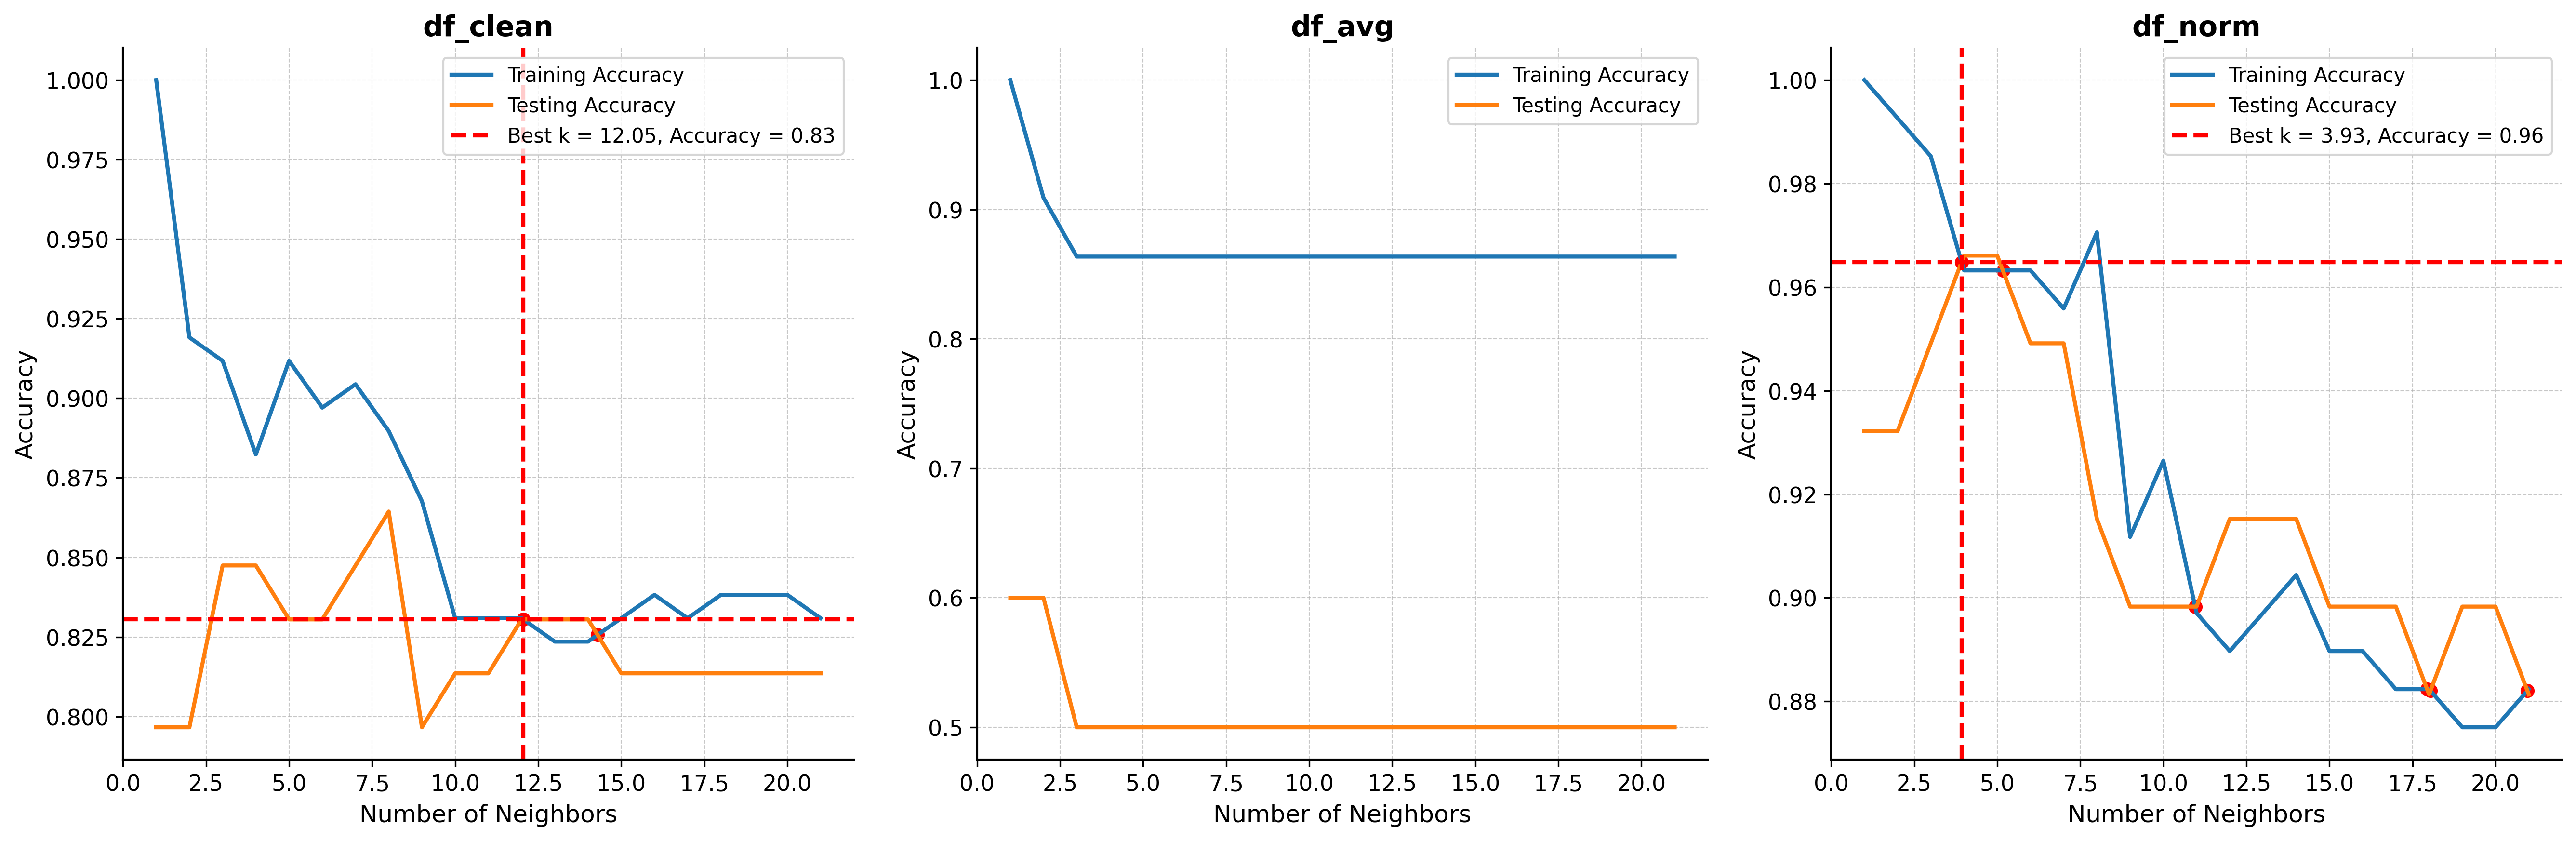
\includegraphics[width=0.99\textwidth]{../images/feature_selection/best_k.png}
	\caption{Optimal \(k\) determination using testing and training accuracy.}
	\label{fig:fig3}
\end{figure}

Finally, the last step is to integrate the whole process within an API. The
backend of this system is implemented using FastAPI. Its primary functions
include serving the frontend, managing model files, retrieving evaluation
metrics, and handling prediction requests, as shown in \cref{fig:fig4}. The
root endpoint (\texttt{/}) serves the \texttt{index.html} file, which provides
the user interface for interaction. The system organizes models into
datetime-labeled folders under \texttt{MODEL\_DIR}, where each folder
represents a distinct training session and contains model files (\texttt{.pkl})
and evaluation metrics stored in a \texttt{metrics.txt} file.

\begin{figure}[H]
	\centering
	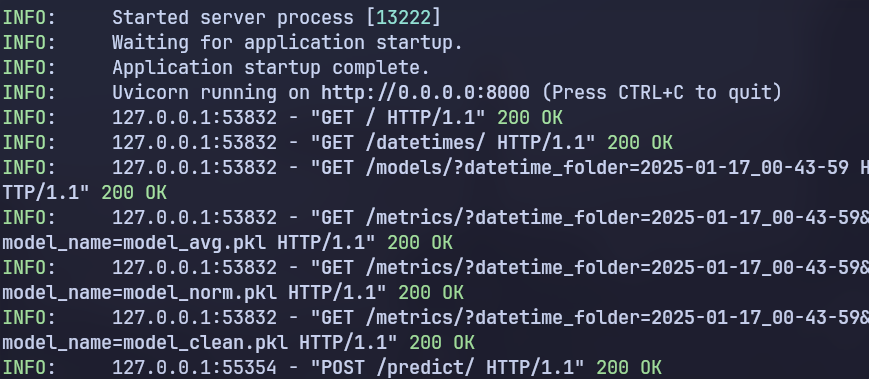
\includegraphics[width=0.80\textwidth,
		height=0.23\textheight]{../images/api/backend.png}
	\caption{Example of messages exchange between frontend and backend.}
	\label{fig:fig4}
\end{figure}

The \texttt{/datetimes/} endpoint retrieves all datetime-named folders,
enabling users to explore different model versions. Once a folder is selected,
the \texttt{/models/} endpoint lists available model files within it. The
\texttt{/metrics/} endpoint fetches and displays the content of the
\texttt{metrics.txt} file for the chosen folder, allowing users to view the
performance metrics of the associated models. The prediction process is handled
by the \texttt{/predict/} endpoint, where the user provides feature inputs and
selects a model. The backend then loads the specified model using the
\texttt{pickle} module and if the selected model is \texttt{model\_norm} it
applies min-max normalization, using pre-computed max-min values from the
normalized dataset. Predictions are generated by the model and returned as a
JSON response, indicating whether the input data corresponds to a healthy or
Parkinson's individual.

The frontend was built using HTML, CSS, and JavaScript. \cref{fig:fig5} shows a
preview of it. Users can select datetime folders and models through dynamically
populated dropdown menus, which are updated by fetching data from the backend
endpoints \texttt{/datetimes/} and \texttt{/models/}. Additionally, users can
upload a JSON file containing feature values, and the uploaded data
automatically populates the input fields, simplifying the data entry process.
Metrics for the selected model are retrieved via the \texttt{/metrics/}
endpoint and displayed directly on the page to provide insights into the
model's performance.

\begin{figure}[H]
	\centering
	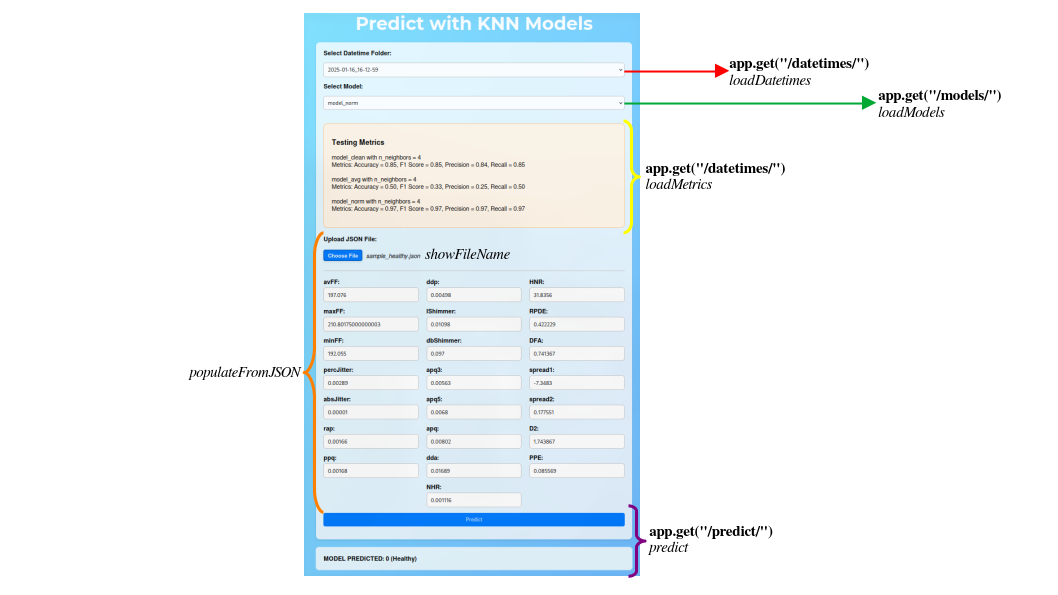
\includegraphics[width=0.95\textwidth,height=0.40\textheight]{../images/api/frontend.png}
	\caption{Frontend preview with annotated elements: functions related to the
		backend are shown in \textbf{bold}, while functions specific to the frontend
		are highlighted in \textit{italics}.}
	\label{fig:fig5}
\end{figure}

The frontend handles form submissions by sending a POST request to the
\texttt{/predict/} endpoint with the user-provided inputs and the selected
model. The backend processes the request, and the prediction results are
displayed directly on the webpage. JavaScript functions manage dynamic
interactions, such as loading datetime folders, model files, and metrics, as
well as validating uploaded JSON files and showing prediction outputs.
